

\begin{frame}
Various Approaches to Covariance Simulation
\begin{itemize}
  \item In the continuous formulation, covariance extrapolation can be accomplished by solving the linear variance equation 
\begin{equation}\label{lvteqcont}
\lveqcont
\end{equation} 
  \item This can be useful in exploring how a navigation system "coasts" in the absence of measurements
	\begin{itemize}
  		\item It can give you an idea of how fast the solution degrades in free-inertial
	\end{itemize}
\end{itemize} 
\end{frame}


\begin{frame}
Various Approaches to Covariance Simulation
\begin{itemize}
  \item In the continuous case, we can also eliminate the gain because
\[\lim_{\Delta t\rightarrow 0}\dfrac{K(t)}{\Delta t}=PH\trans R^{-1}\]
  \item This leads to a single equation, the Matrix Riccati equation, for covariance propadation and update:
\begin{equation}\label{matrixriccatieq}
\matrixriccatieq
\end{equation} 
\end{itemize} 
\end{frame}

\begin{frame}[fragile]
Various Approaches to Covariance Simulation
\begin{itemize}
  \item Matrix Riccati Equation reveals essential characteristics of filter
\[\matrixriccatieq\]
  \item Note that in this equation we increase estimation uncertainty by adding in process noise
  \item And we decrease estimation uncertainty by the amount of information ($R^{-1}$) inherent in the measurement 
\end{itemize} 
\end{frame}
\begin{frame}[fragile]
Various Approaches to Covariance Simulation
\begin{itemize}
  \item See Matlab / Simulink Model \begin{verbatim}matrix_riccati.mdl\end{verbatim}
  \item Dampled harmonic oscillator; parameter file \begin{verbatim}harmosc_riccati.mat\end{verbatim}
	\begin{itemize}
		\item 2d state vector: position and velocity
		\item 1 scalar measurement and scalar measurement noise $R$
	\end{itemize}
\end{itemize} 
\end{frame}

\begin{frame}

\begin{center}
%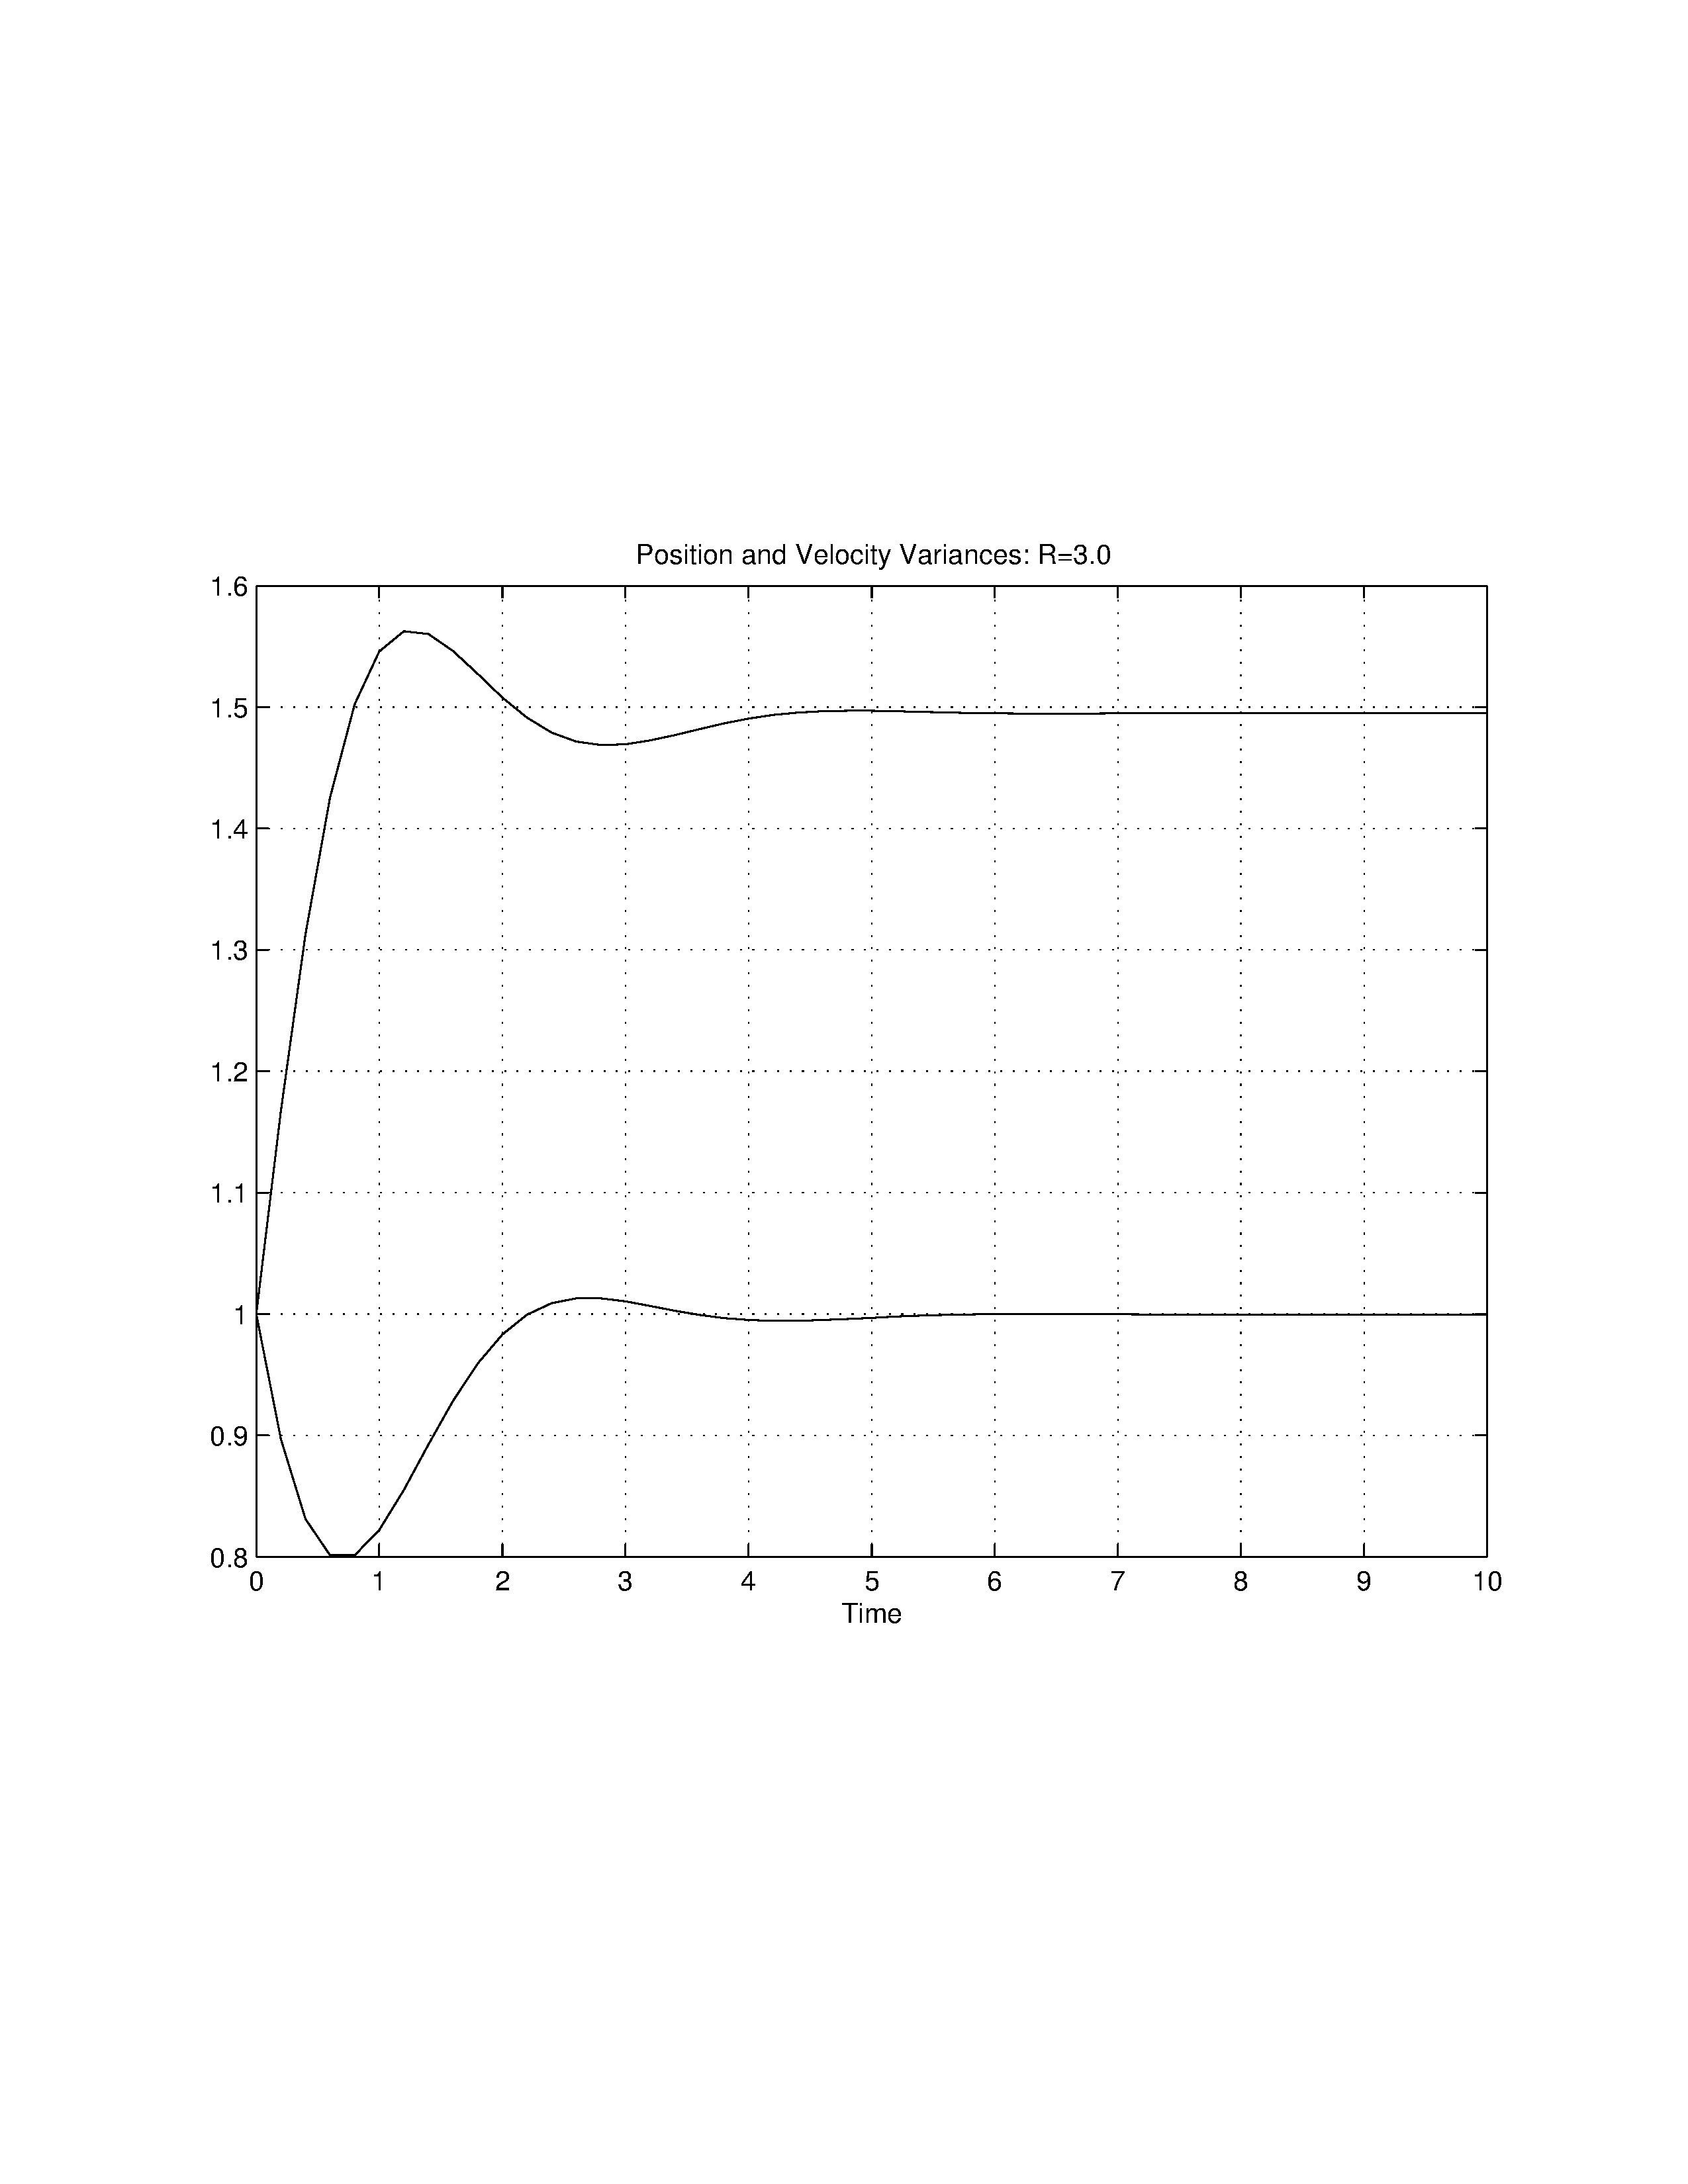
\includegraphics[width=.80\textwidth]{matlab/harmosc_riccati_fig1.jpg}
\end{center}
\end{frame}


\begin{frame}
\begin{center}
%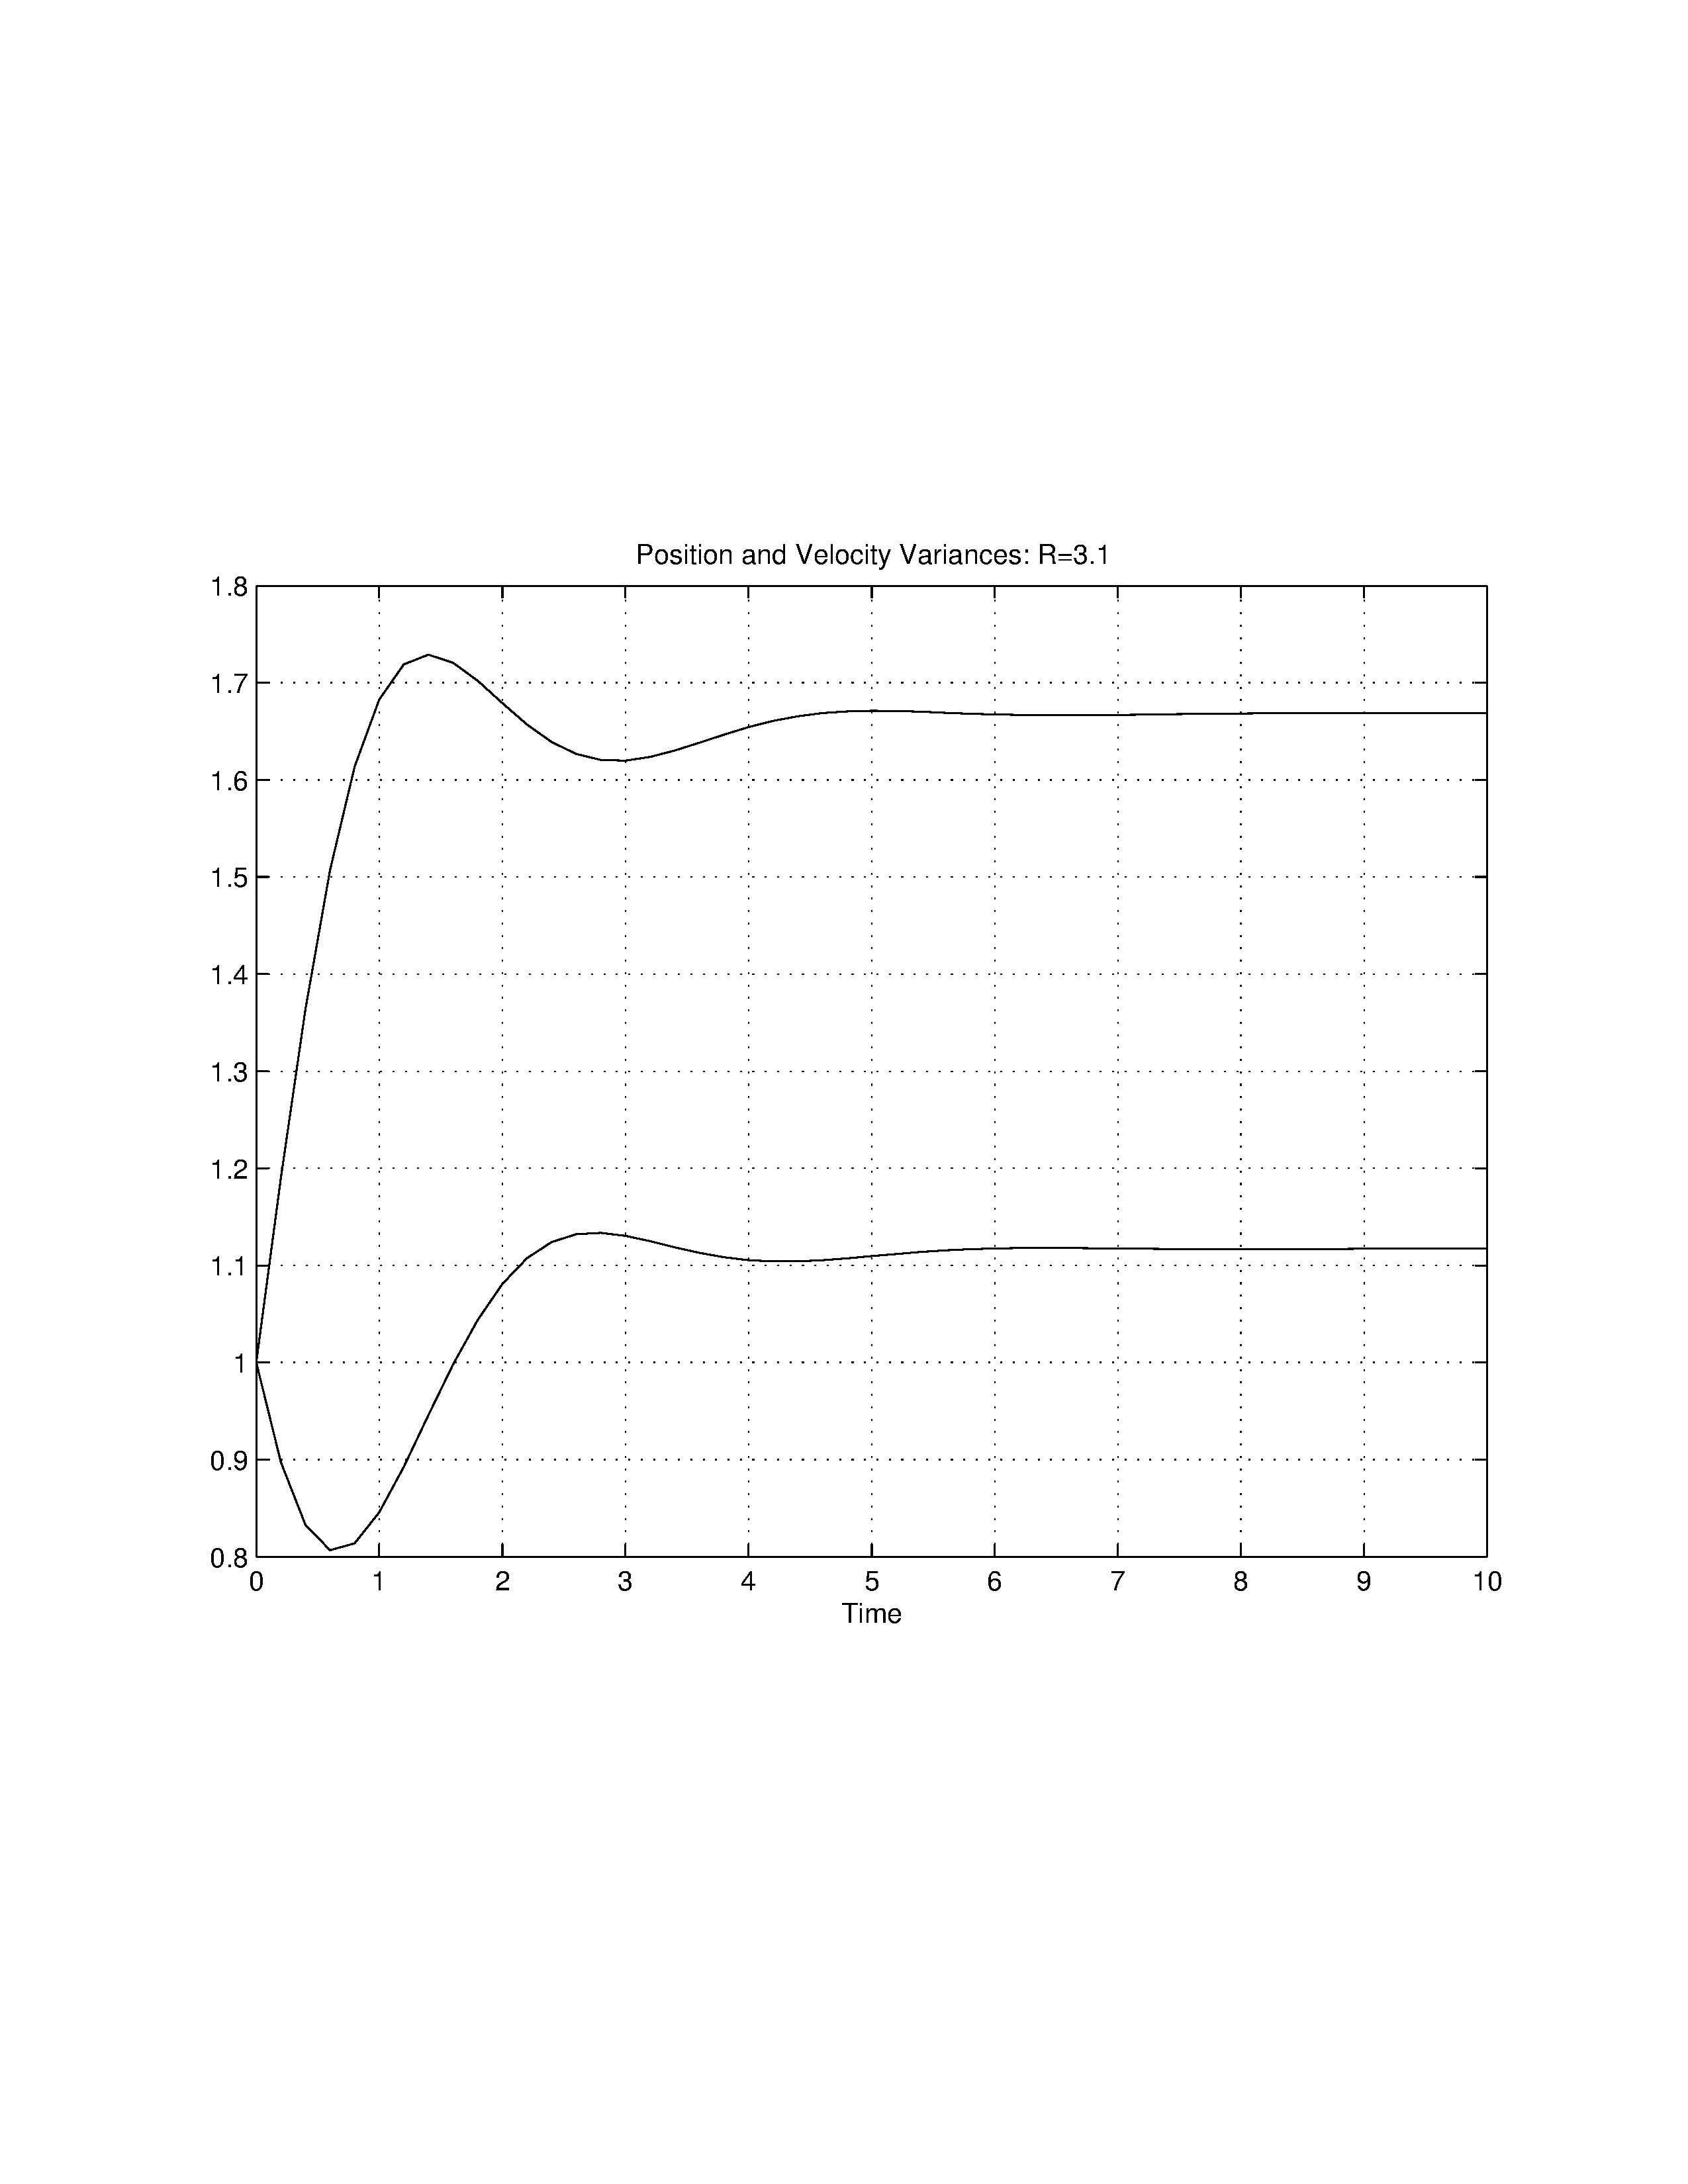
\includegraphics[width=.80\textwidth]{matlab/harmosc_riccati_fig2.jpg}
\end{center}
\end{frame}

\begin{frame}
\begin{center}
%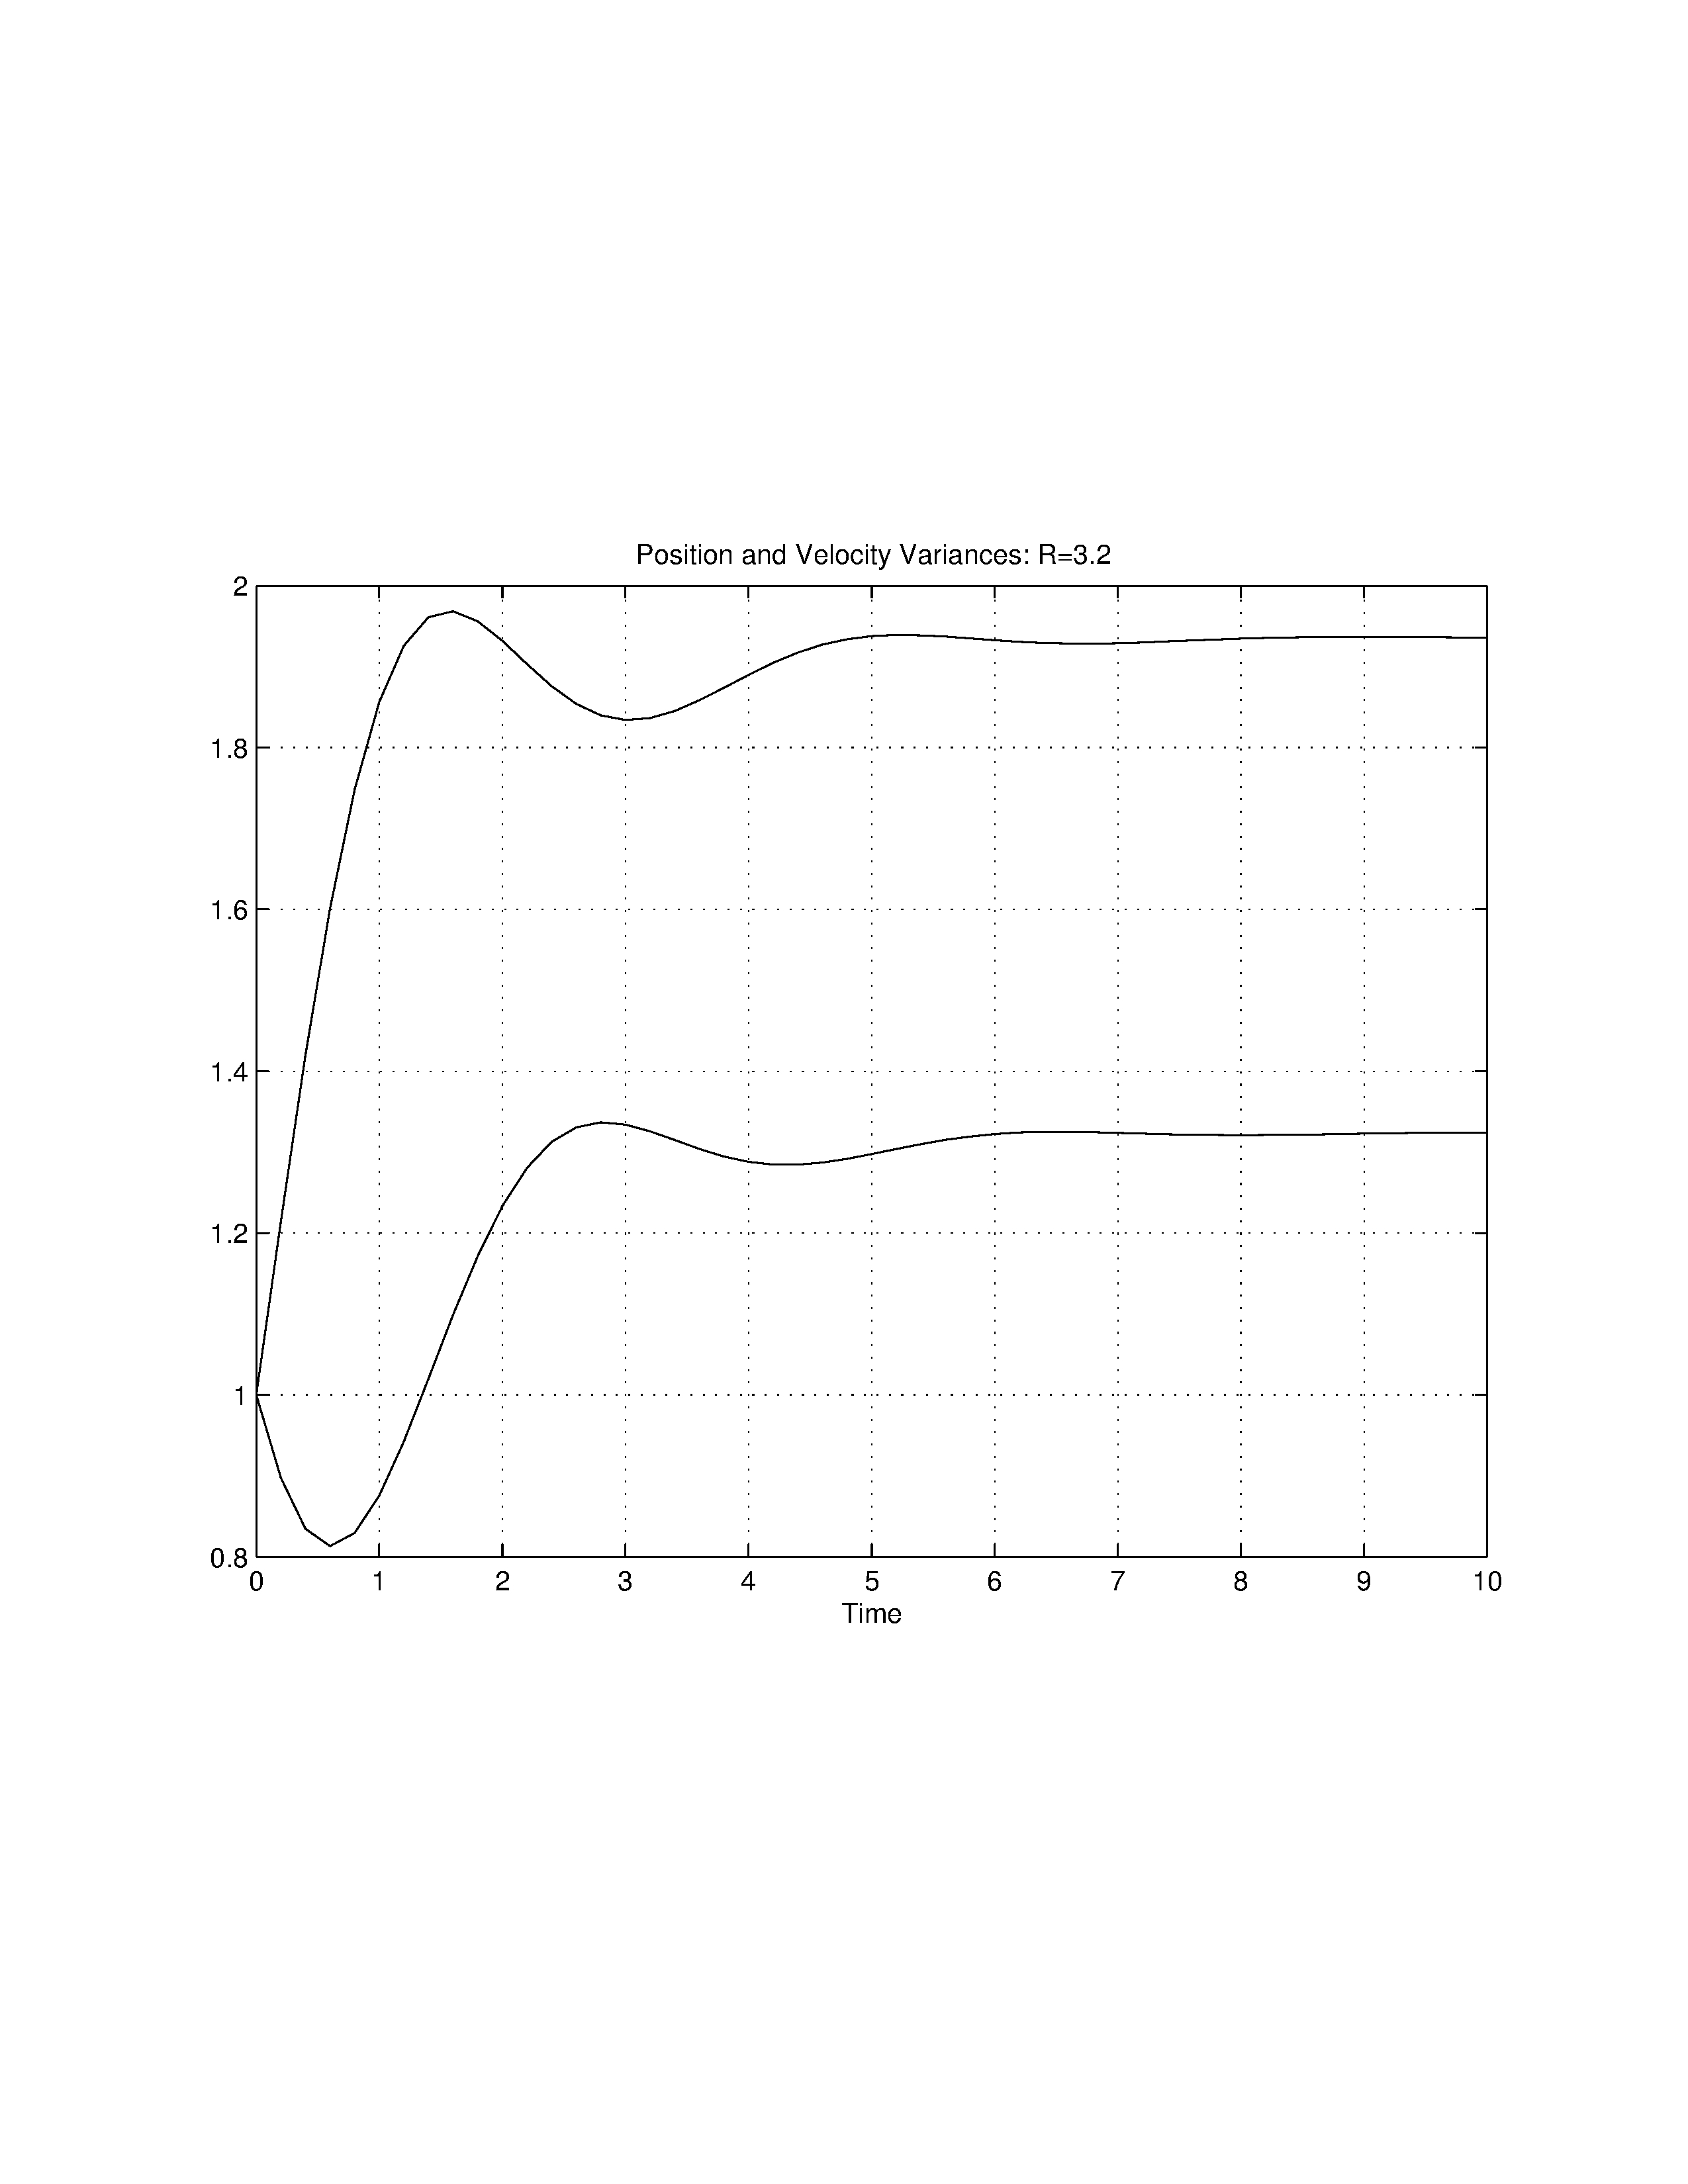
\includegraphics[width=.80\textwidth]{matlab/harmosc_riccati_fig3.jpg}
\end{center}
\end{frame}


\begin{frame}
\begin{center}
%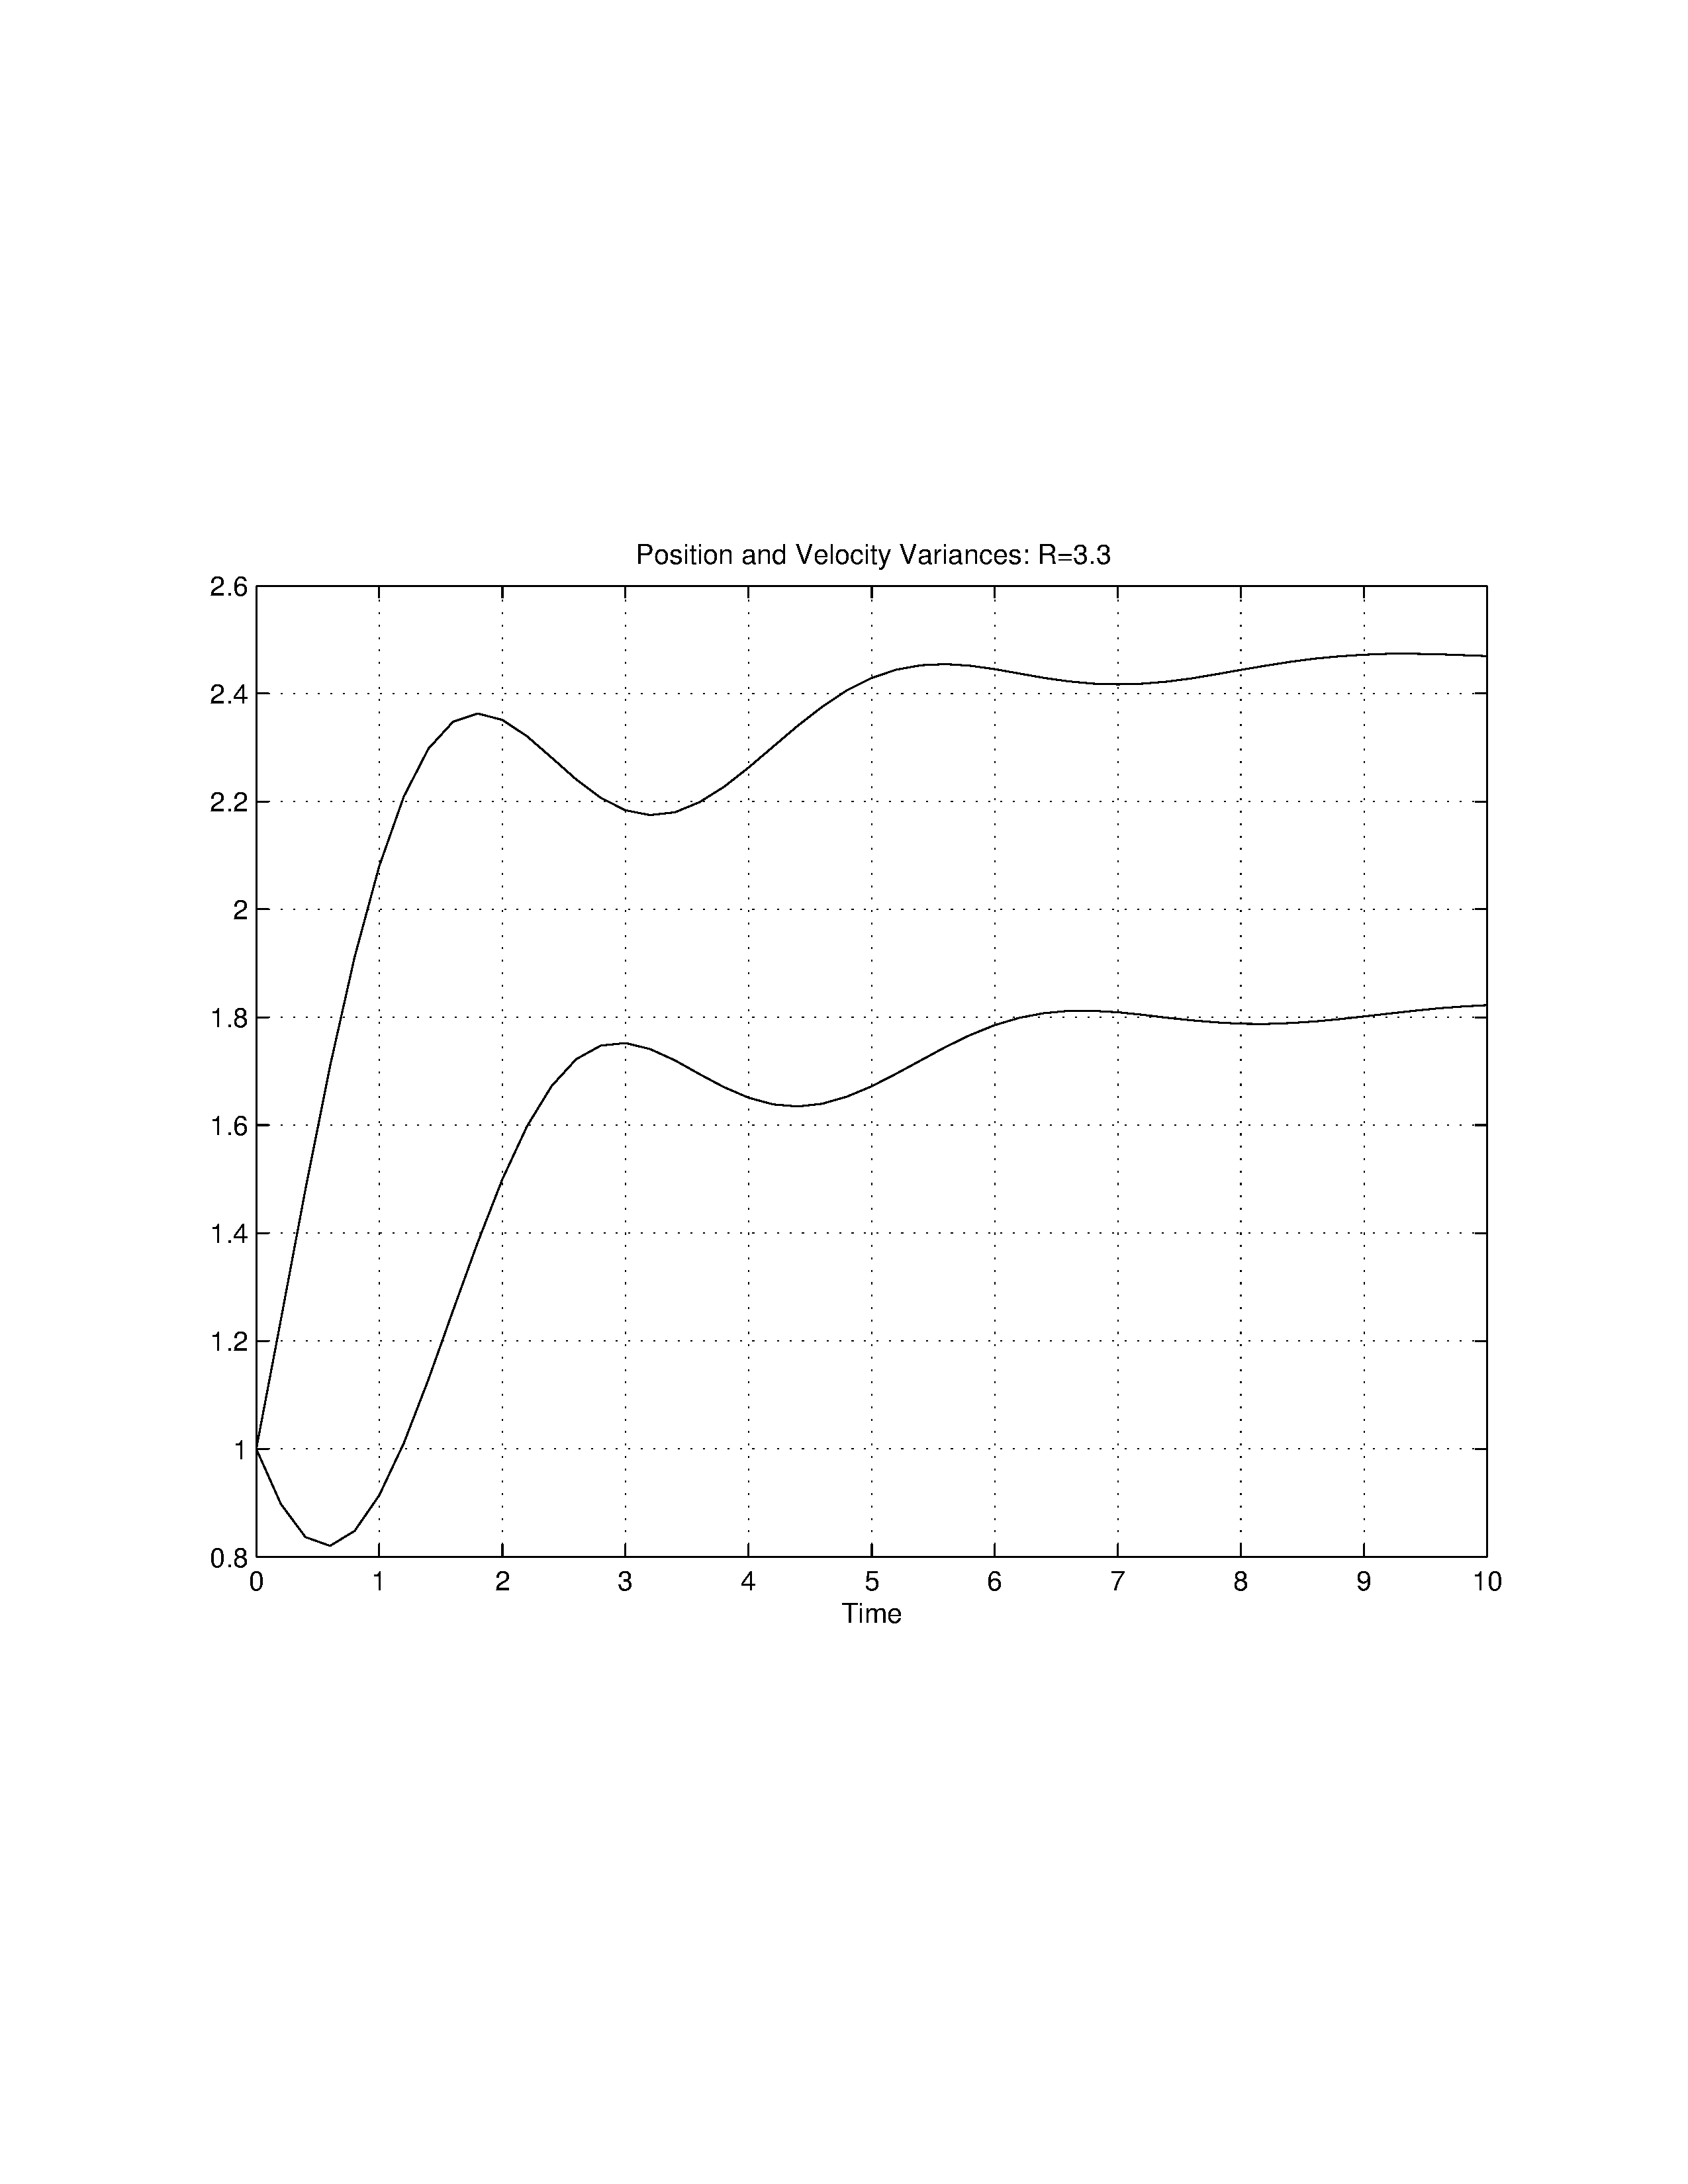
\includegraphics[width=.80\textwidth]{matlab/harmosc_riccati_fig4.jpg}
\end{center}
\end{frame}

\begin{frame}
\begin{center}
%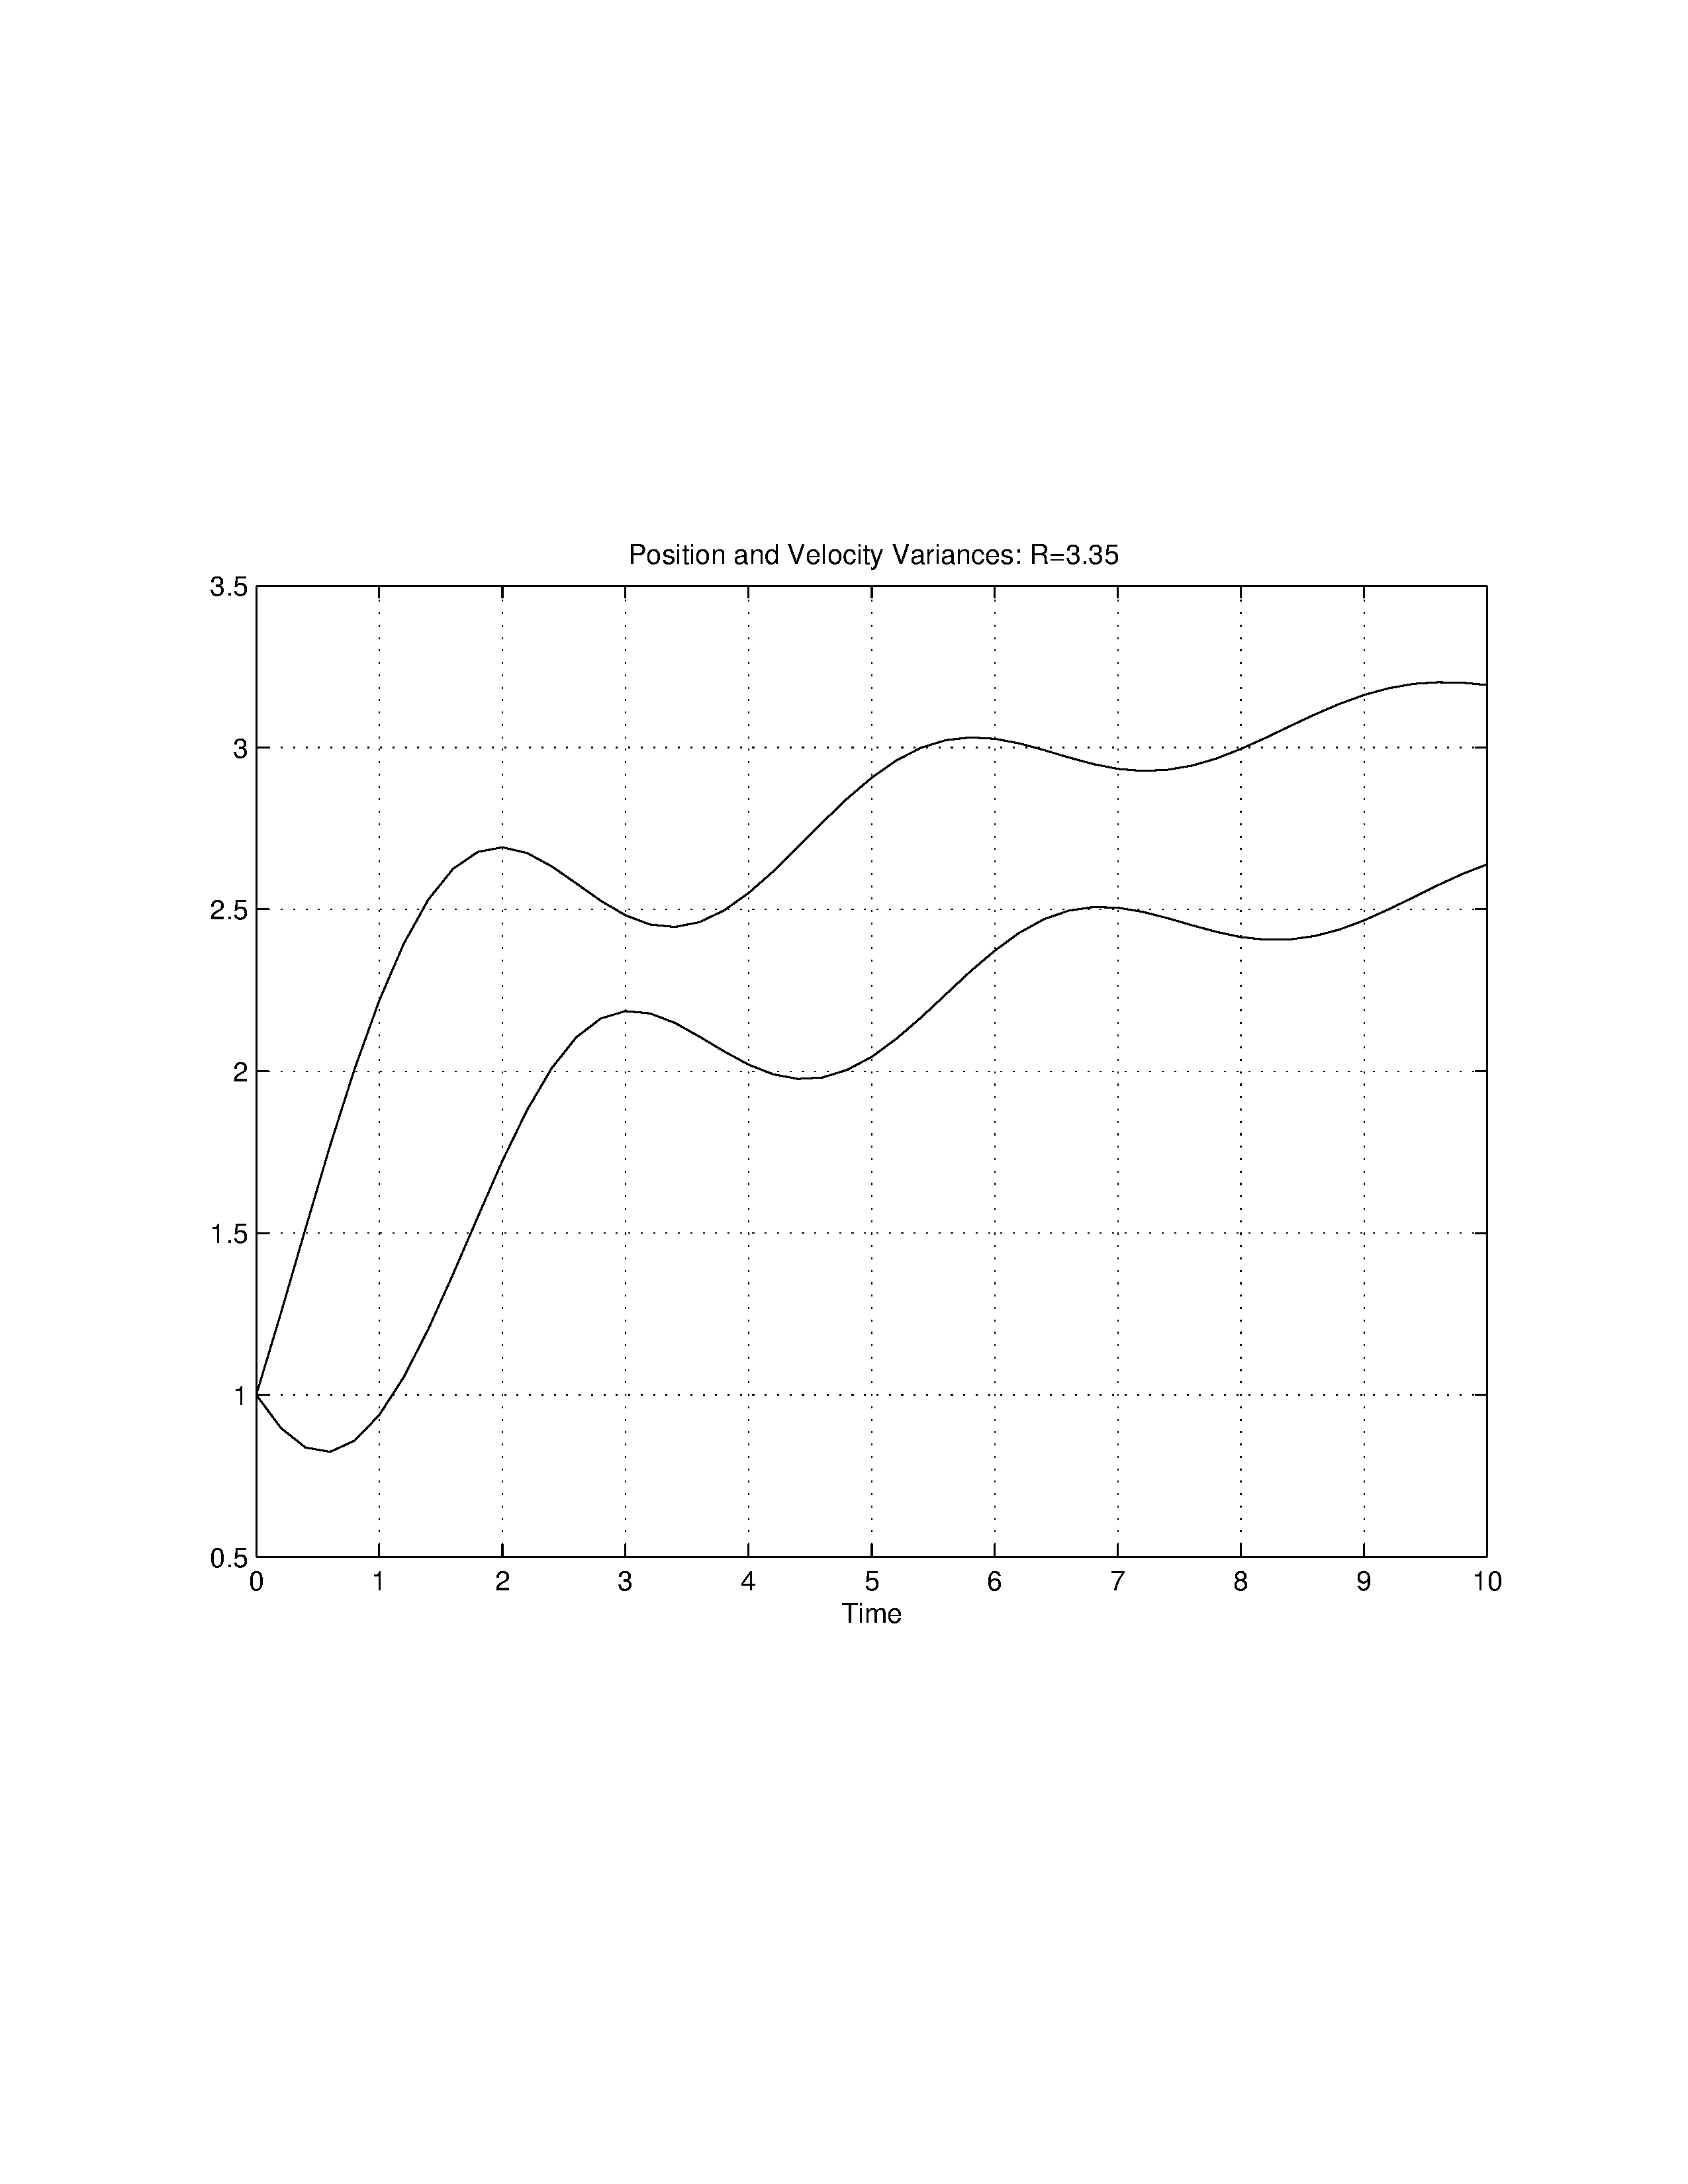
\includegraphics[width=.80\textwidth]{matlab/harmosc_riccati_fig5.jpg}
\end{center}
\end{frame}

\begin{frame}
\begin{center}
%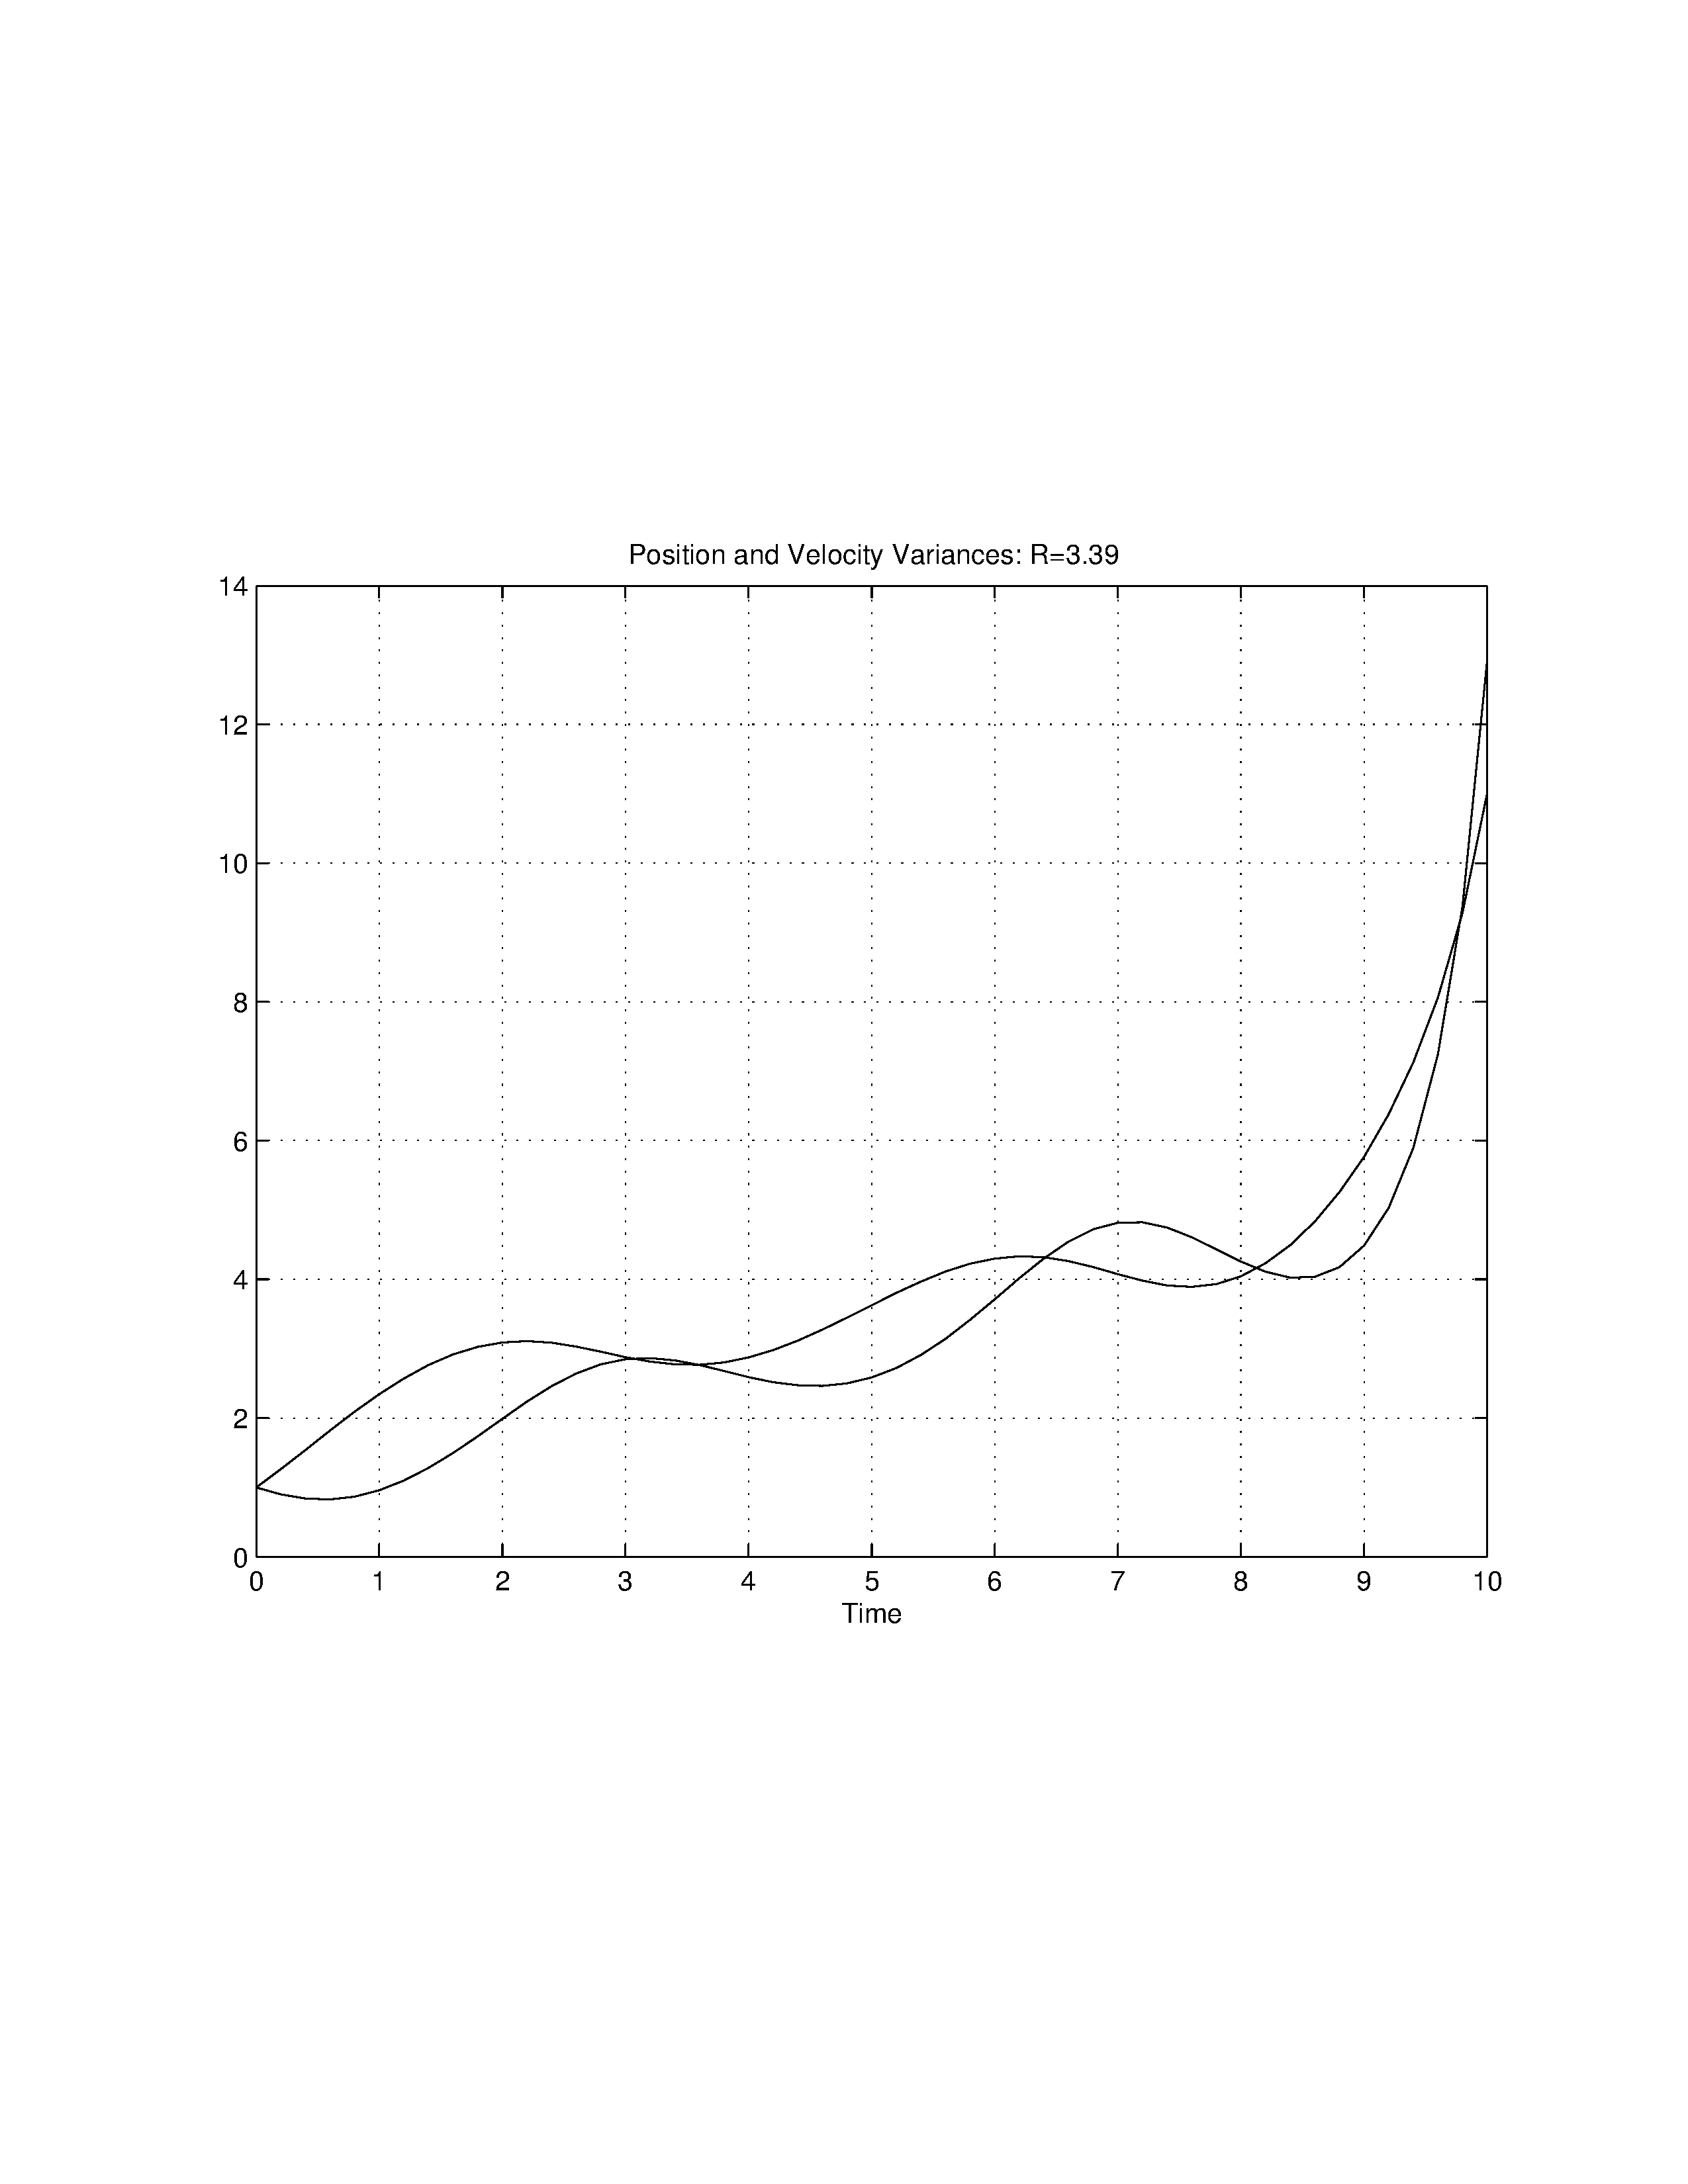
\includegraphics[width=.80\textwidth]{matlab/harmosc_riccati_fig6.jpg}
\end{center}
\end{frame}

\begin{frame}
Damped Harmonic Oscillator Covariance Analysis
\begin{itemize}
  \item Matrix Riccati Differential Equation with constant $F$, $H$, $Q$, $R$
  \item Varying $R$ demonstrates extreme sensivitiy of $P$ solution to changes in $R$
  \item $R=3.3$ is stable; but $R=3.4$ is unstable
\end{itemize} 
\end{frame}

\begin{frame}
Damped Harmonic Oscillator Covariance Analysis
\begin{itemize}
  \item Example illustrates how damping coefficient (reflected in system dynamics matrix $F$) and process noise uncertainty $Q$ interact with measurement noise uncertainty $R$
  \item Highly coupled, non-linear equation
\end{itemize}
\[\matrixriccatieq\] 
\end{frame}

\begin{frame}
Alternative Forms of Matrix Riccati Equation
\begin{itemize}
  \item Can be factored into two first-order, linear matrix
  \item May be better behaved numerically
	\begin{itemize}
		\item with Matlab / Simulink it is very easy to implment even non-linear matrix differential equations
		\item Simulink's ODE solvers may not always be up to the task, however
	\end{itemize}
\end{itemize} 
\end{frame}


\begin{frame}
Various Approachs to Covariance Simulation
\begin{itemize}
  \item Discrete models:
	\begin{itemize}
		\item Implement regular filter processing less the state propagation and update
	\end{itemize}
\end{itemize} 
\end{frame}

